\section{Screenshots of the Working Analyzer}\label{c:screens}

Captured from the running application by \texttt{capture-report-\allowbreak
screenshots.mjs}, which drives a real browser against the live service. These are not
mock-ups.

\begin{figure}[htbp]
  \centering
  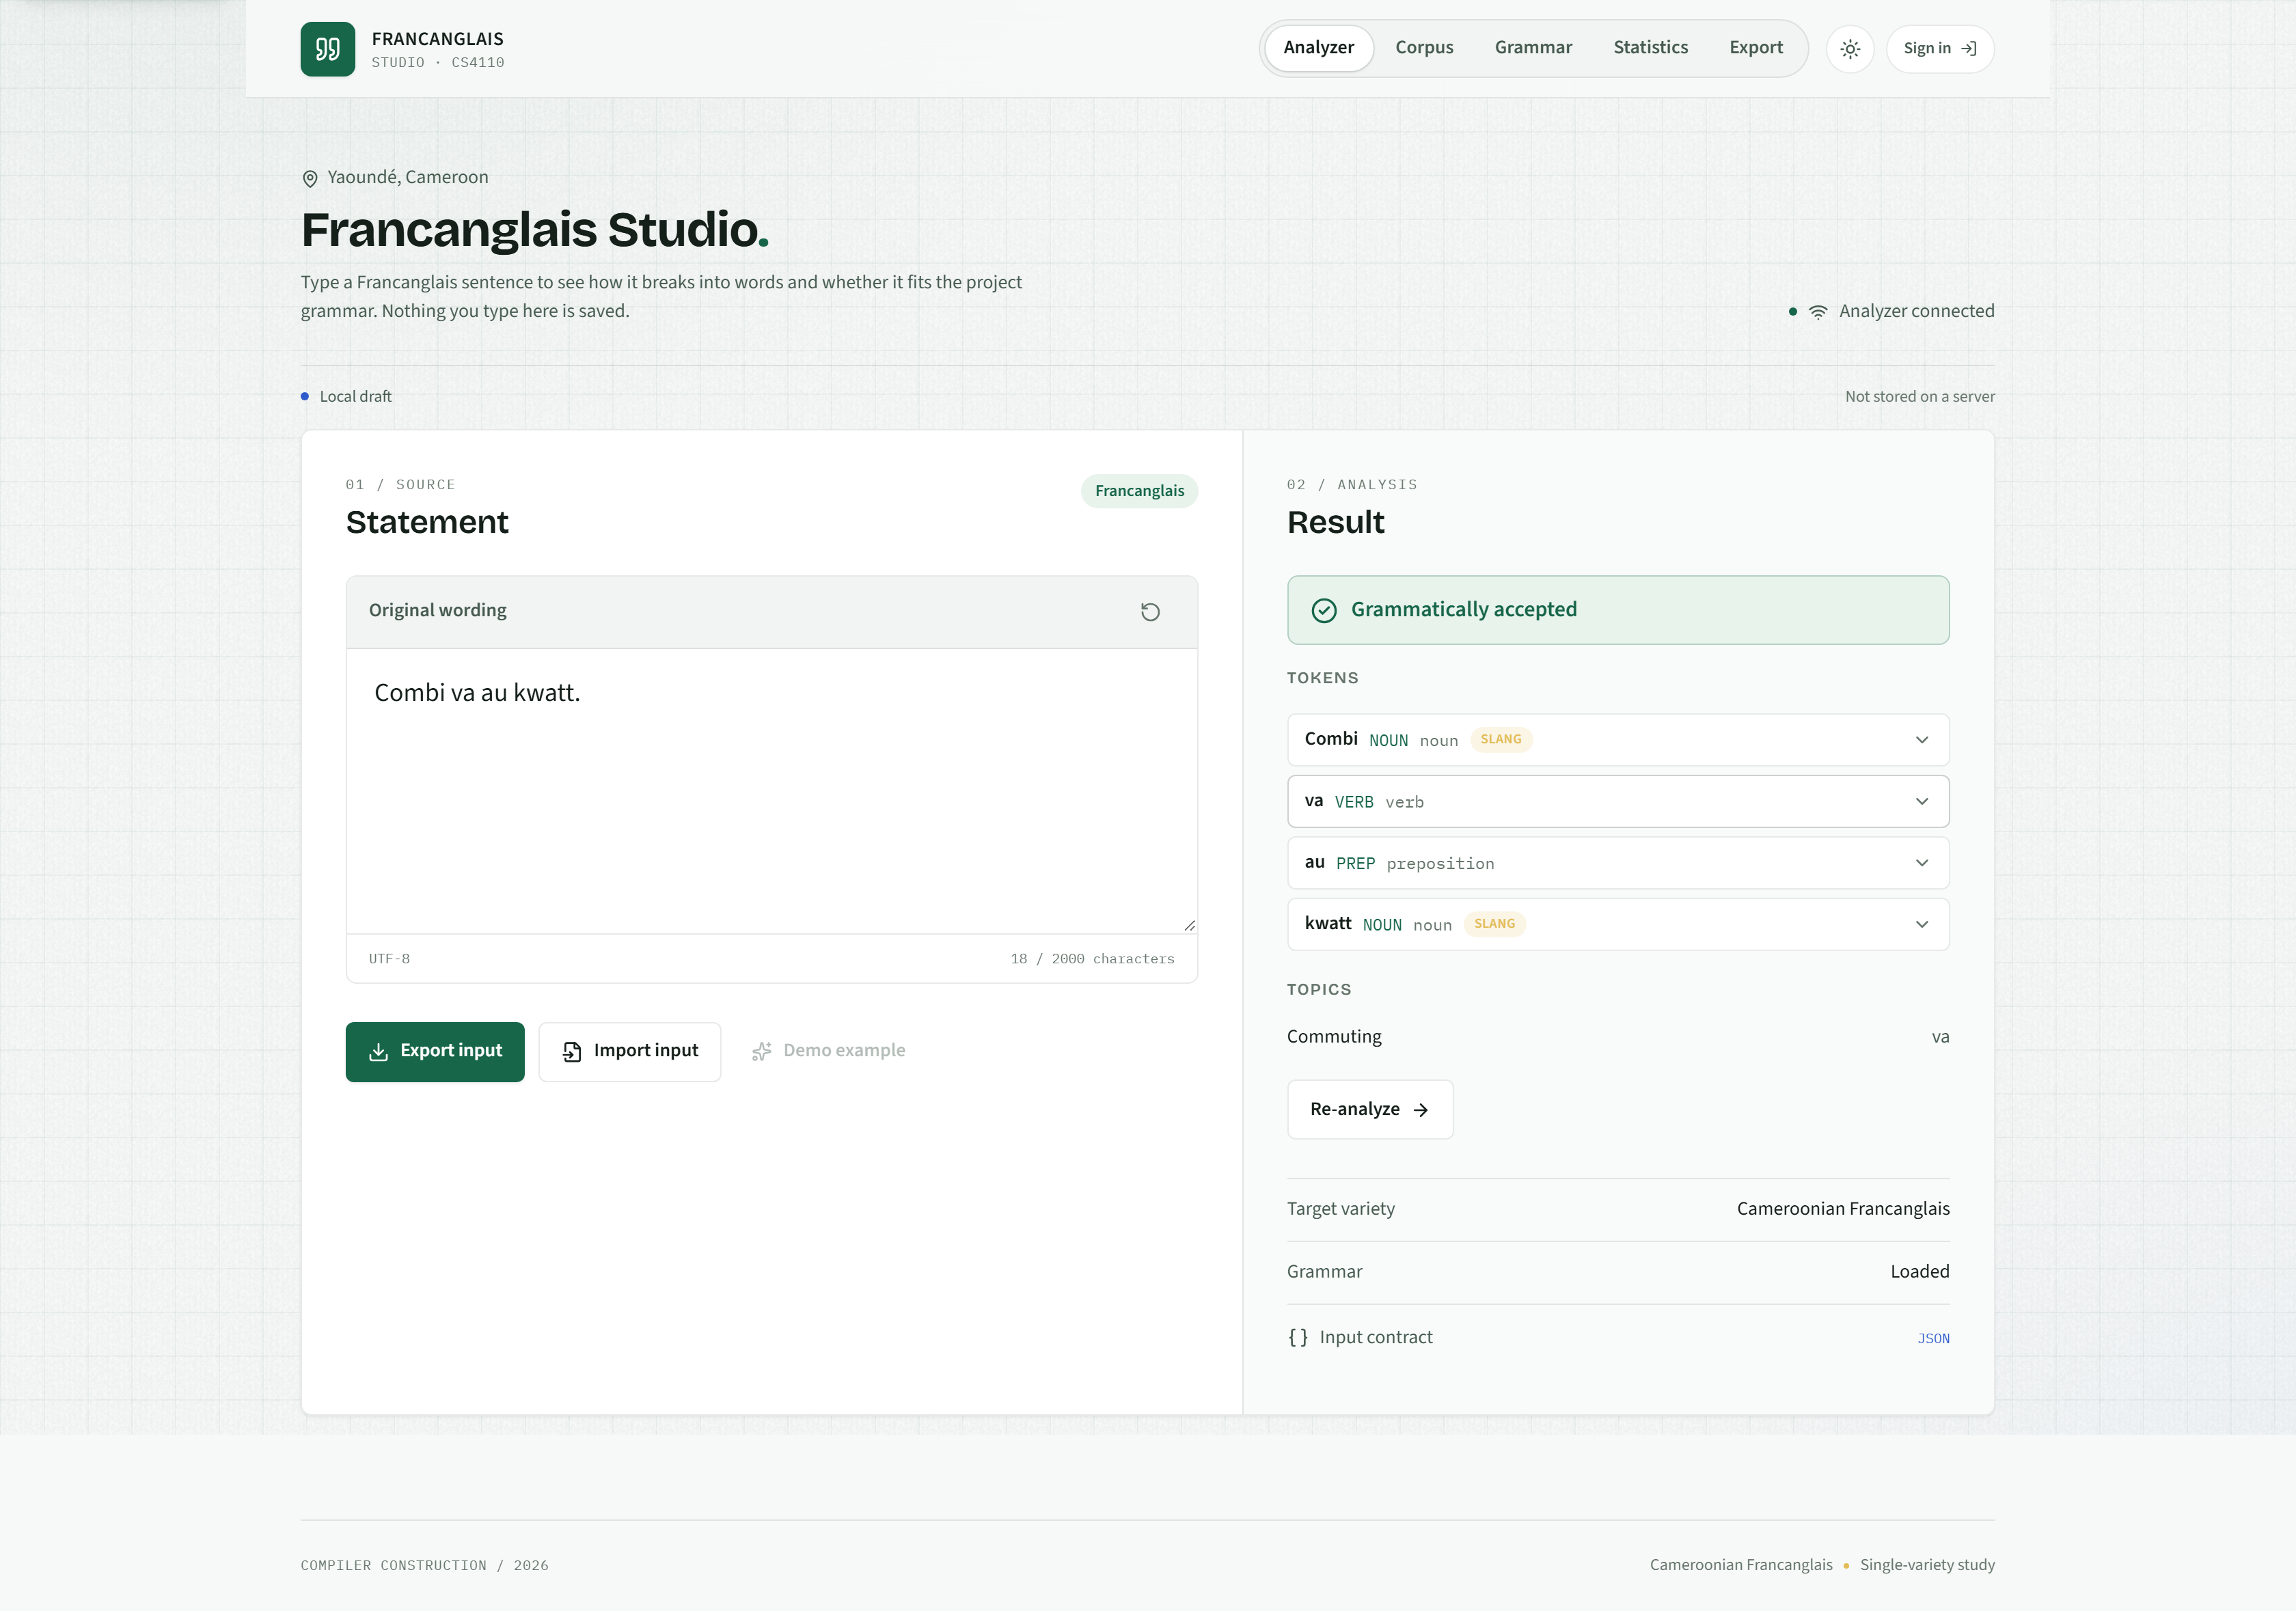
\includegraphics[width=0.78\linewidth]{figures/shot-analyser.png}
  \caption{Analyser view. \fw{Combi va au kwatt.} resolves to \term{NOUN VERB PREP NOUN},
  with \fw{combi} and \fw{kwatt} flagged as slang; the verdict is \accepted\ and the topic
  rule reports \term{commuting}, citing the word that triggered it.}
\end{figure}

\begin{figure}[htbp]
  \centering
  \begin{minipage}[t]{0.49\linewidth}
    \centering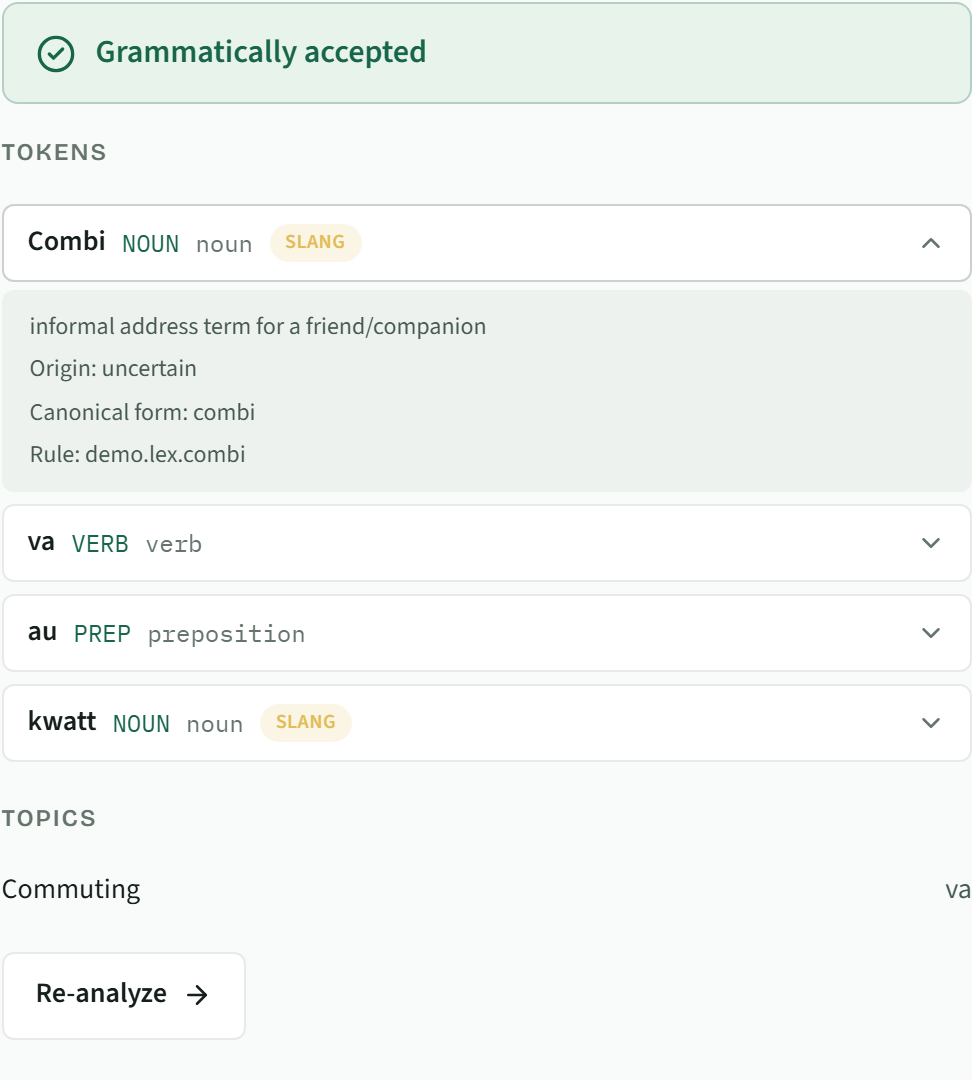
\includegraphics[width=\linewidth]{figures/shot-tokens.png}
  \end{minipage}\hfill
  \begin{minipage}[t]{0.49\linewidth}
    \centering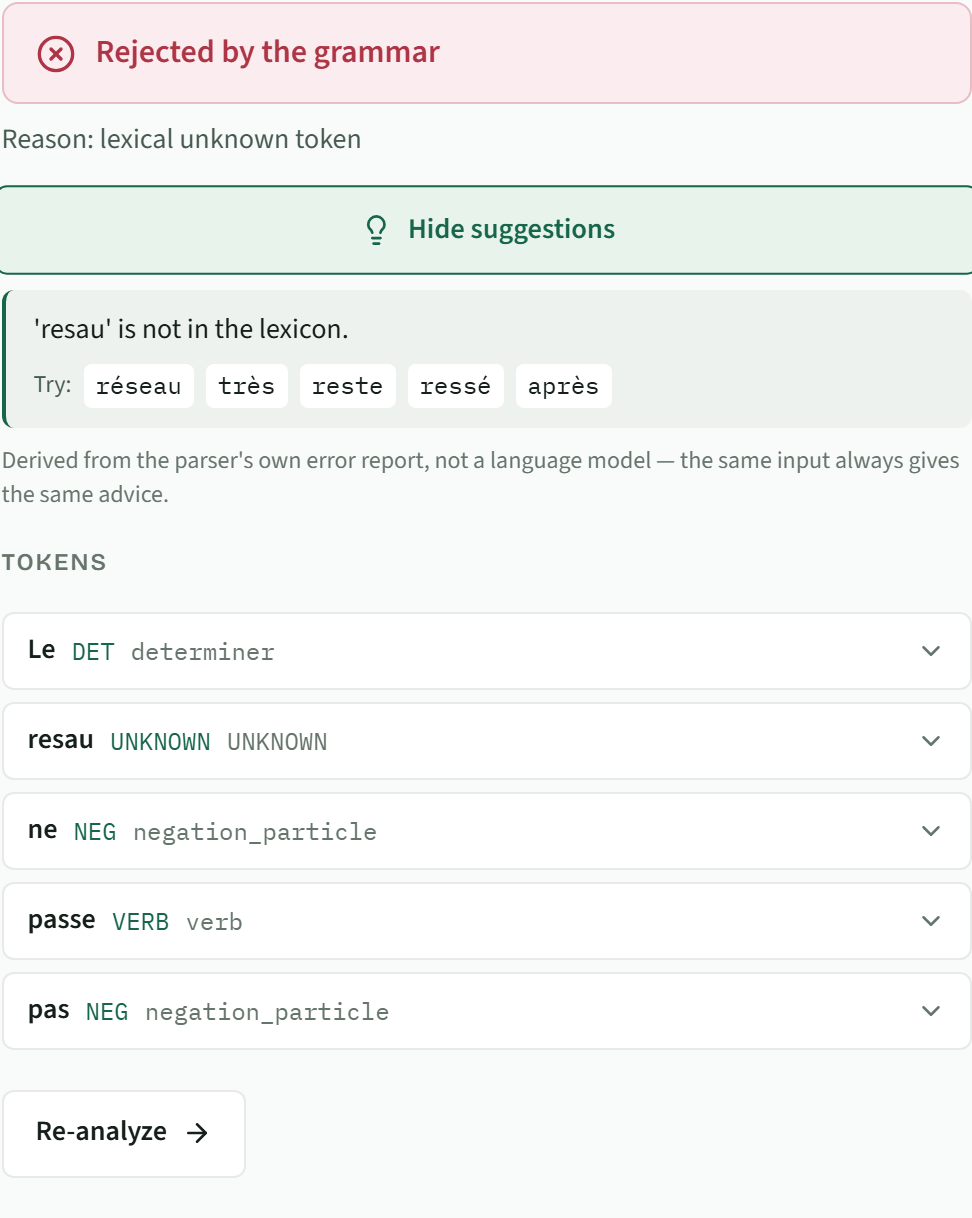
\includegraphics[width=\linewidth]{figures/shot-rejected.png}
  \end{minipage}
  \caption{Left: an expanded token showing canonical form, terminal class, donor language
  and gloss. Right: \fw{Le resau ne passe pas.} \rejected\ with reason
  \term{lexical unknown token}; \emph{Suggest a fix} recovers the intended \fw{réseau}
  despite the missing accent, because matching runs over folded forms.}
\end{figure}

\begin{figure}[htbp]
  \centering
  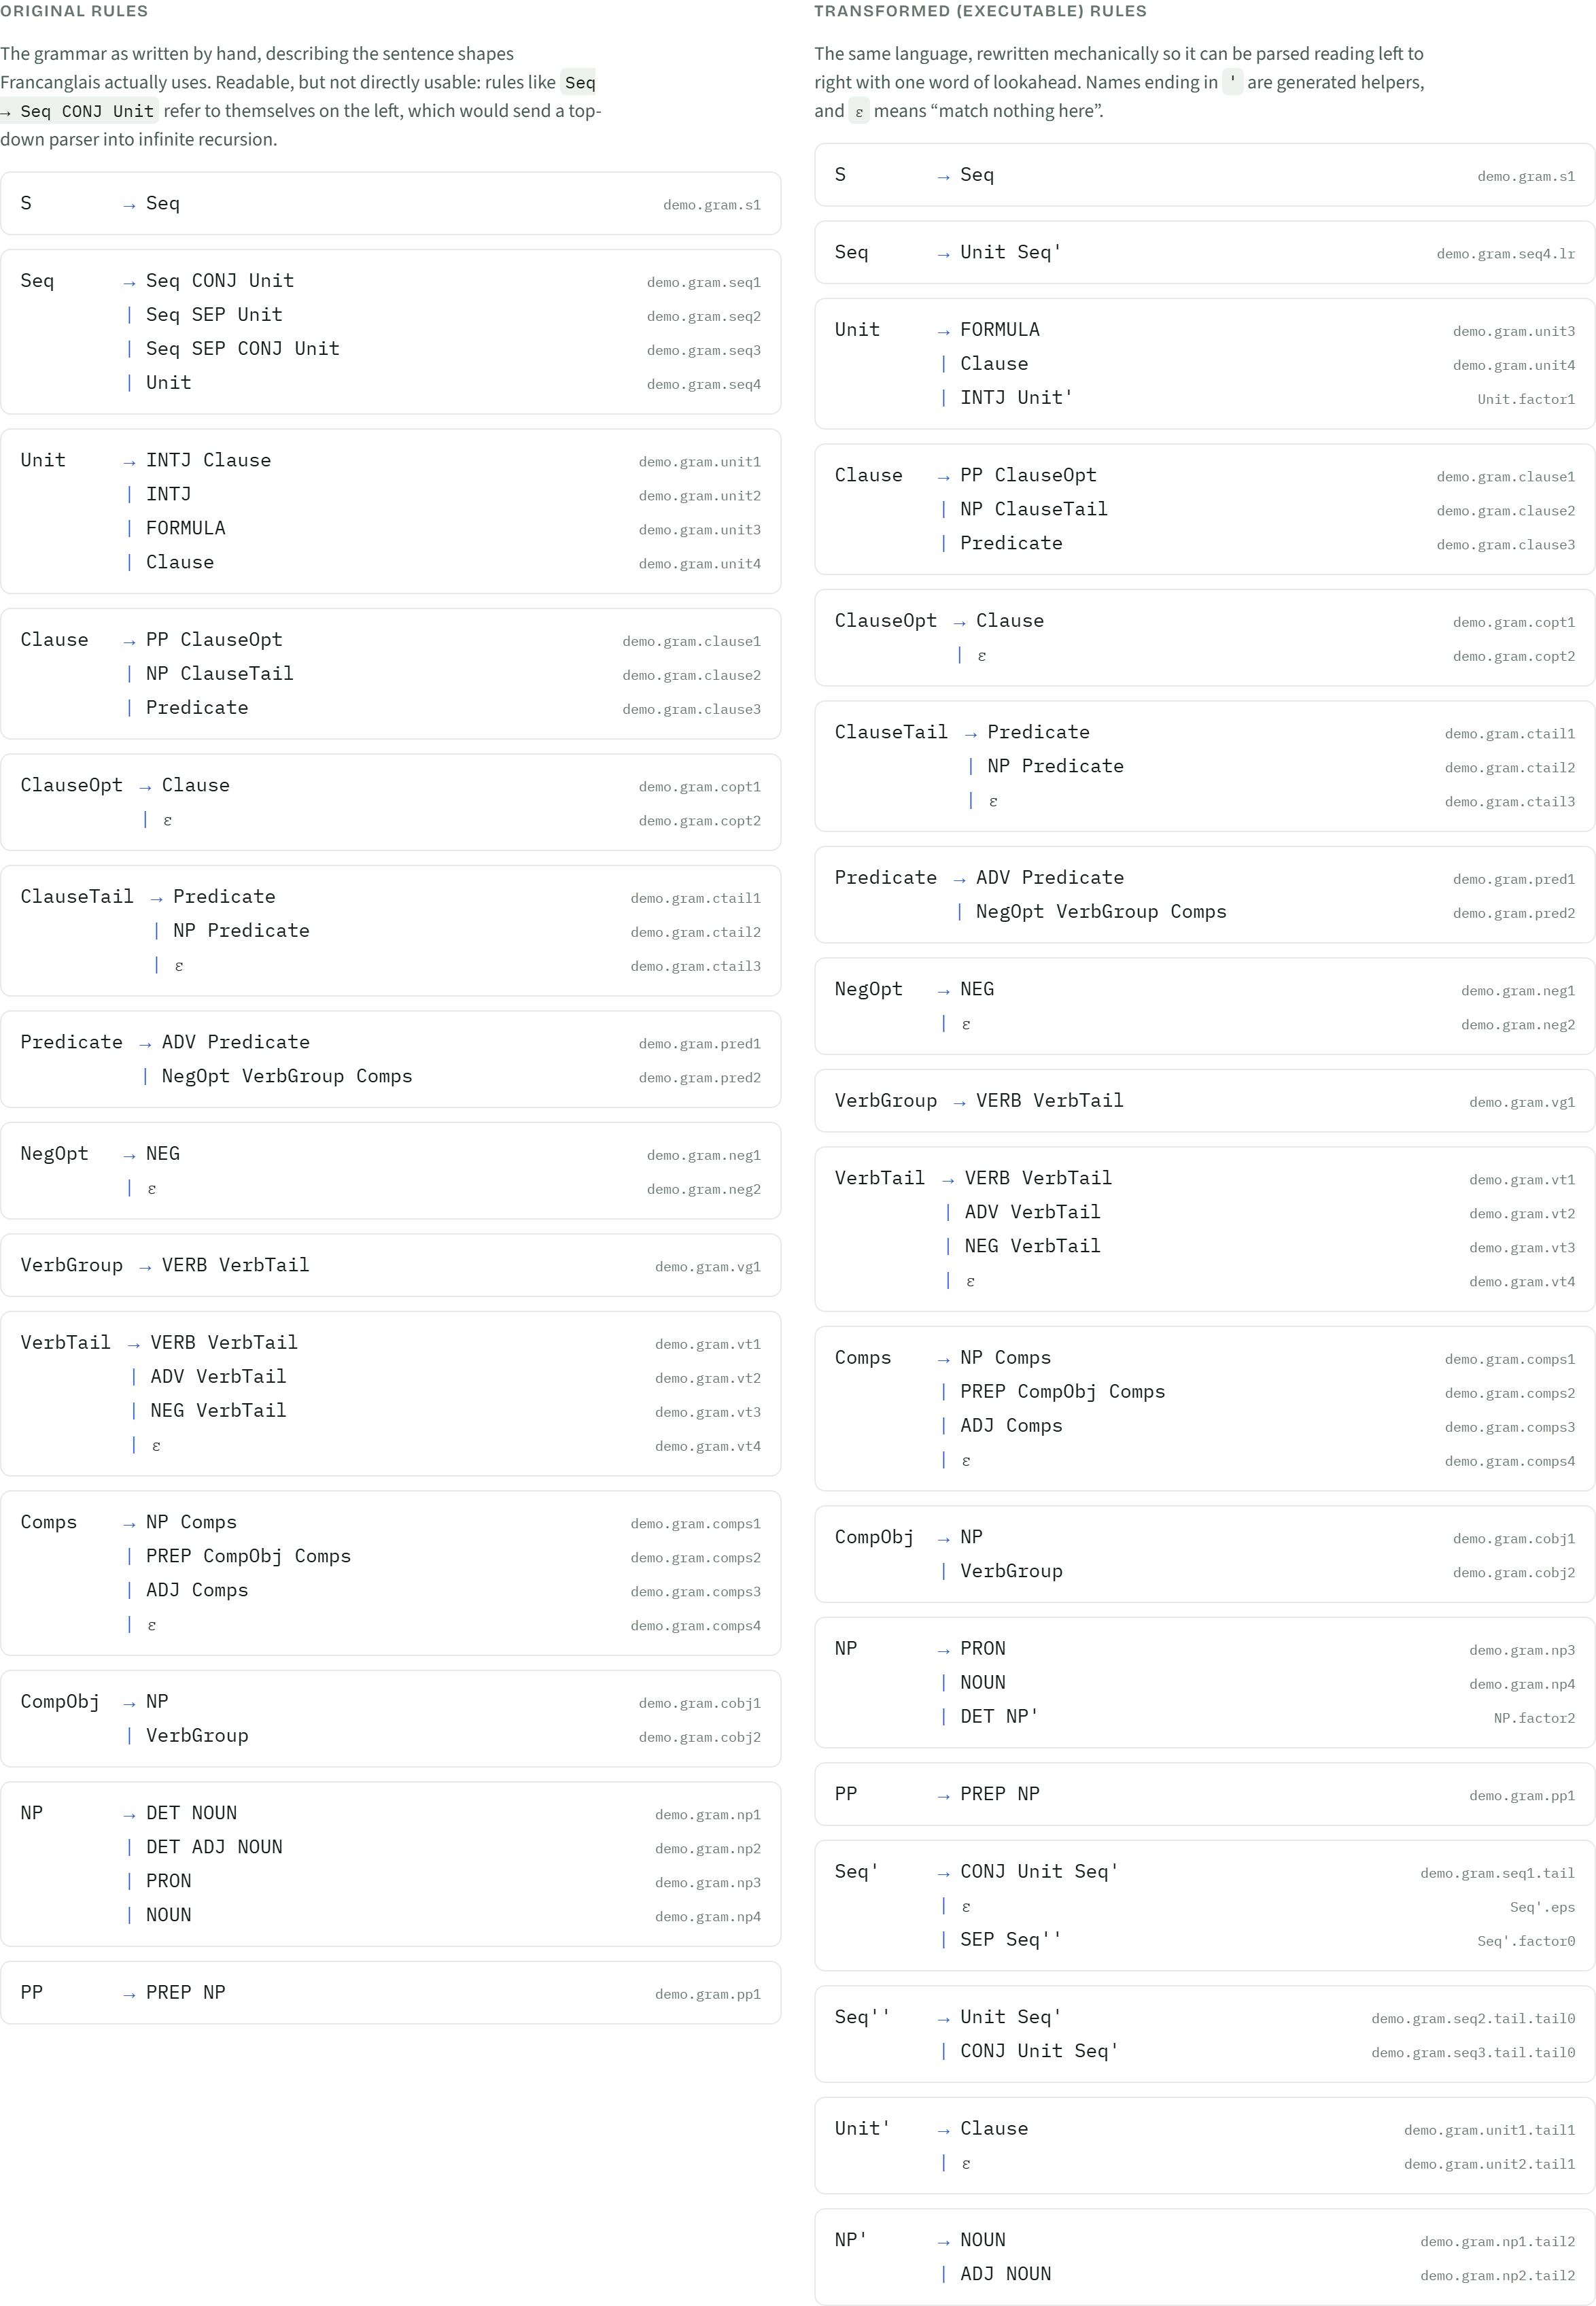
\includegraphics[width=0.88\linewidth]{figures/shot-grammar-original.png}
  \caption{Grammar explorer: the authored left-recursive grammar beside its mechanically
  transformed LL(1) equivalent, with the interface explaining why the rewrite is
  necessary.}
\end{figure}

\begin{figure}[htbp]
  \centering
  \begin{minipage}[t]{0.49\linewidth}
    \centering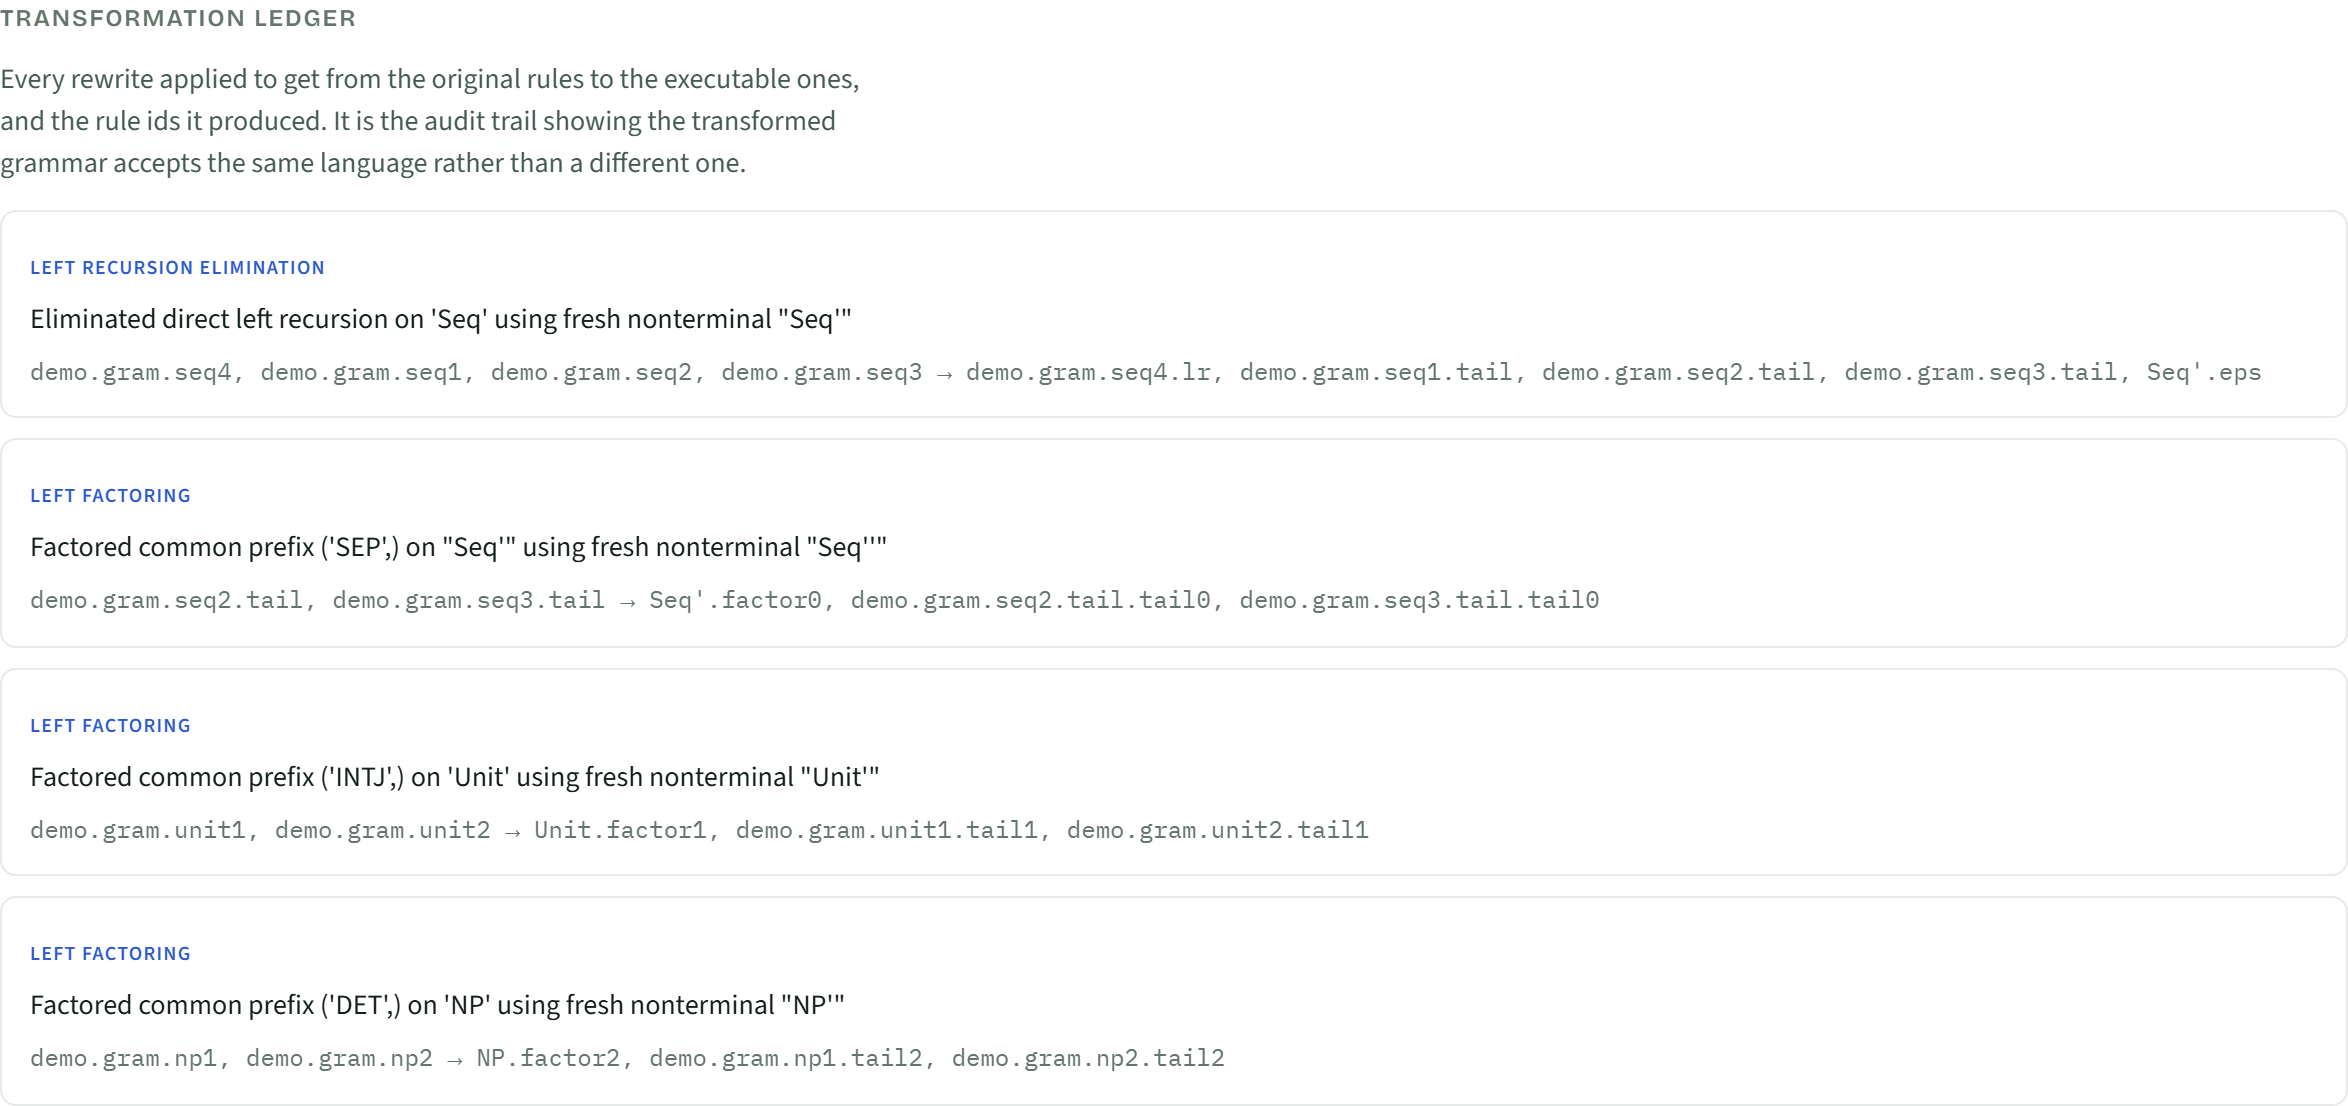
\includegraphics[width=\linewidth]{figures/shot-ledger.png}
  \end{minipage}\hfill
  \begin{minipage}[t]{0.49\linewidth}
    \centering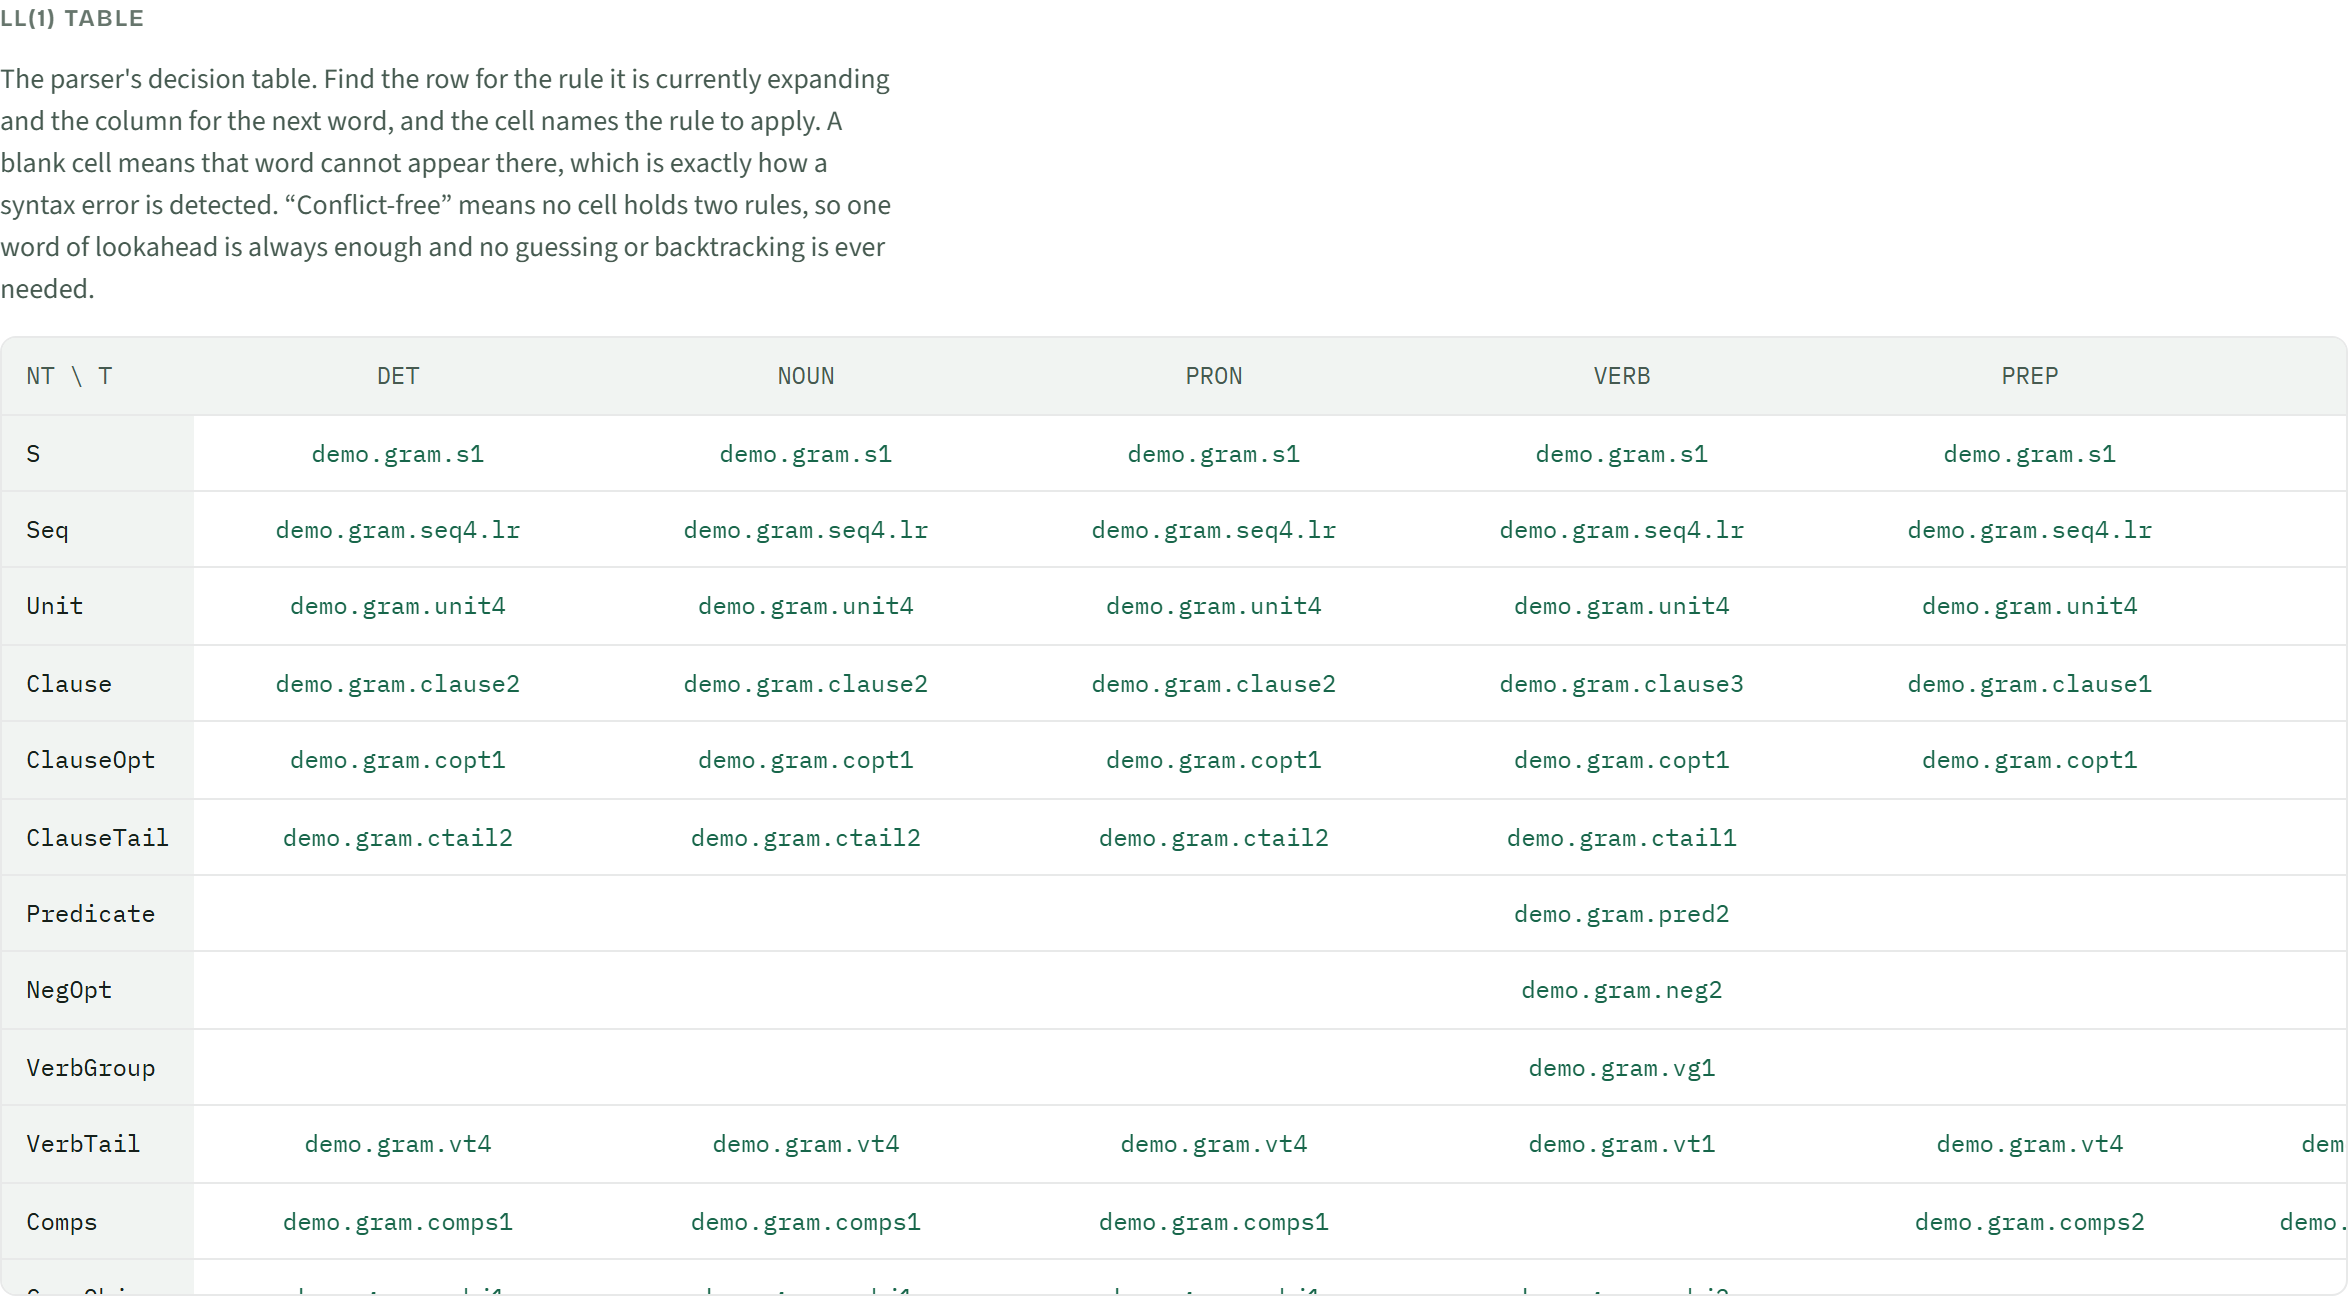
\includegraphics[width=\linewidth]{figures/shot-ll1-table.png}
  \end{minipage}
  \caption{Left: the \LedgerSteps\ recorded transformation steps, each naming the rules
  consumed and produced. Right: the constructed LL(1) parsing table as the interface
  presents it, inside a scrolling pane.}
\end{figure}

\begin{figure}[htbp]
  \centering
  \begin{minipage}[t]{0.47\linewidth}
    \centering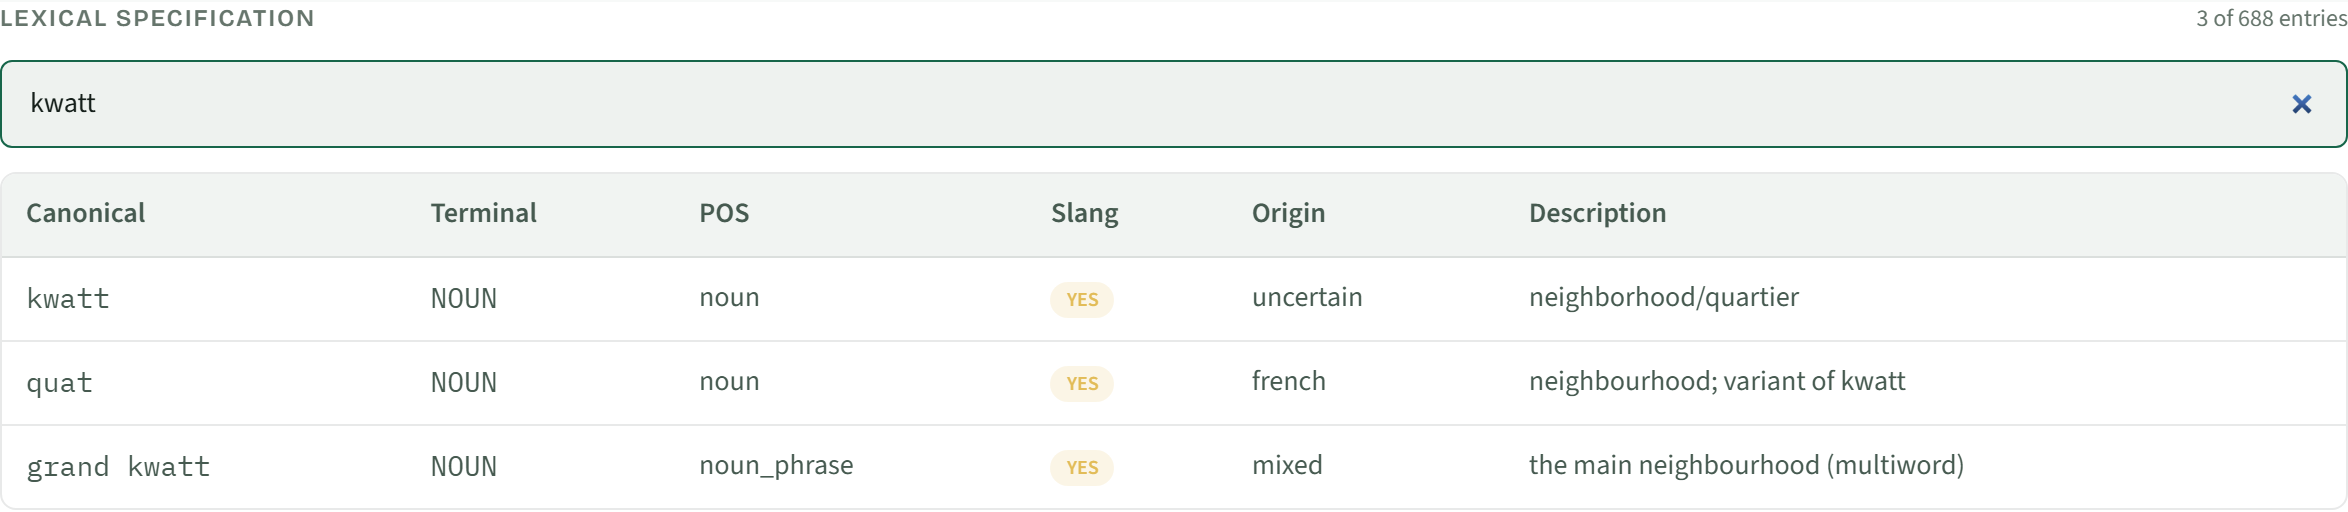
\includegraphics[width=\linewidth]{figures/shot-lexicon-search.png}
  \end{minipage}\hfill
  \begin{minipage}[t]{0.51\linewidth}
    \centering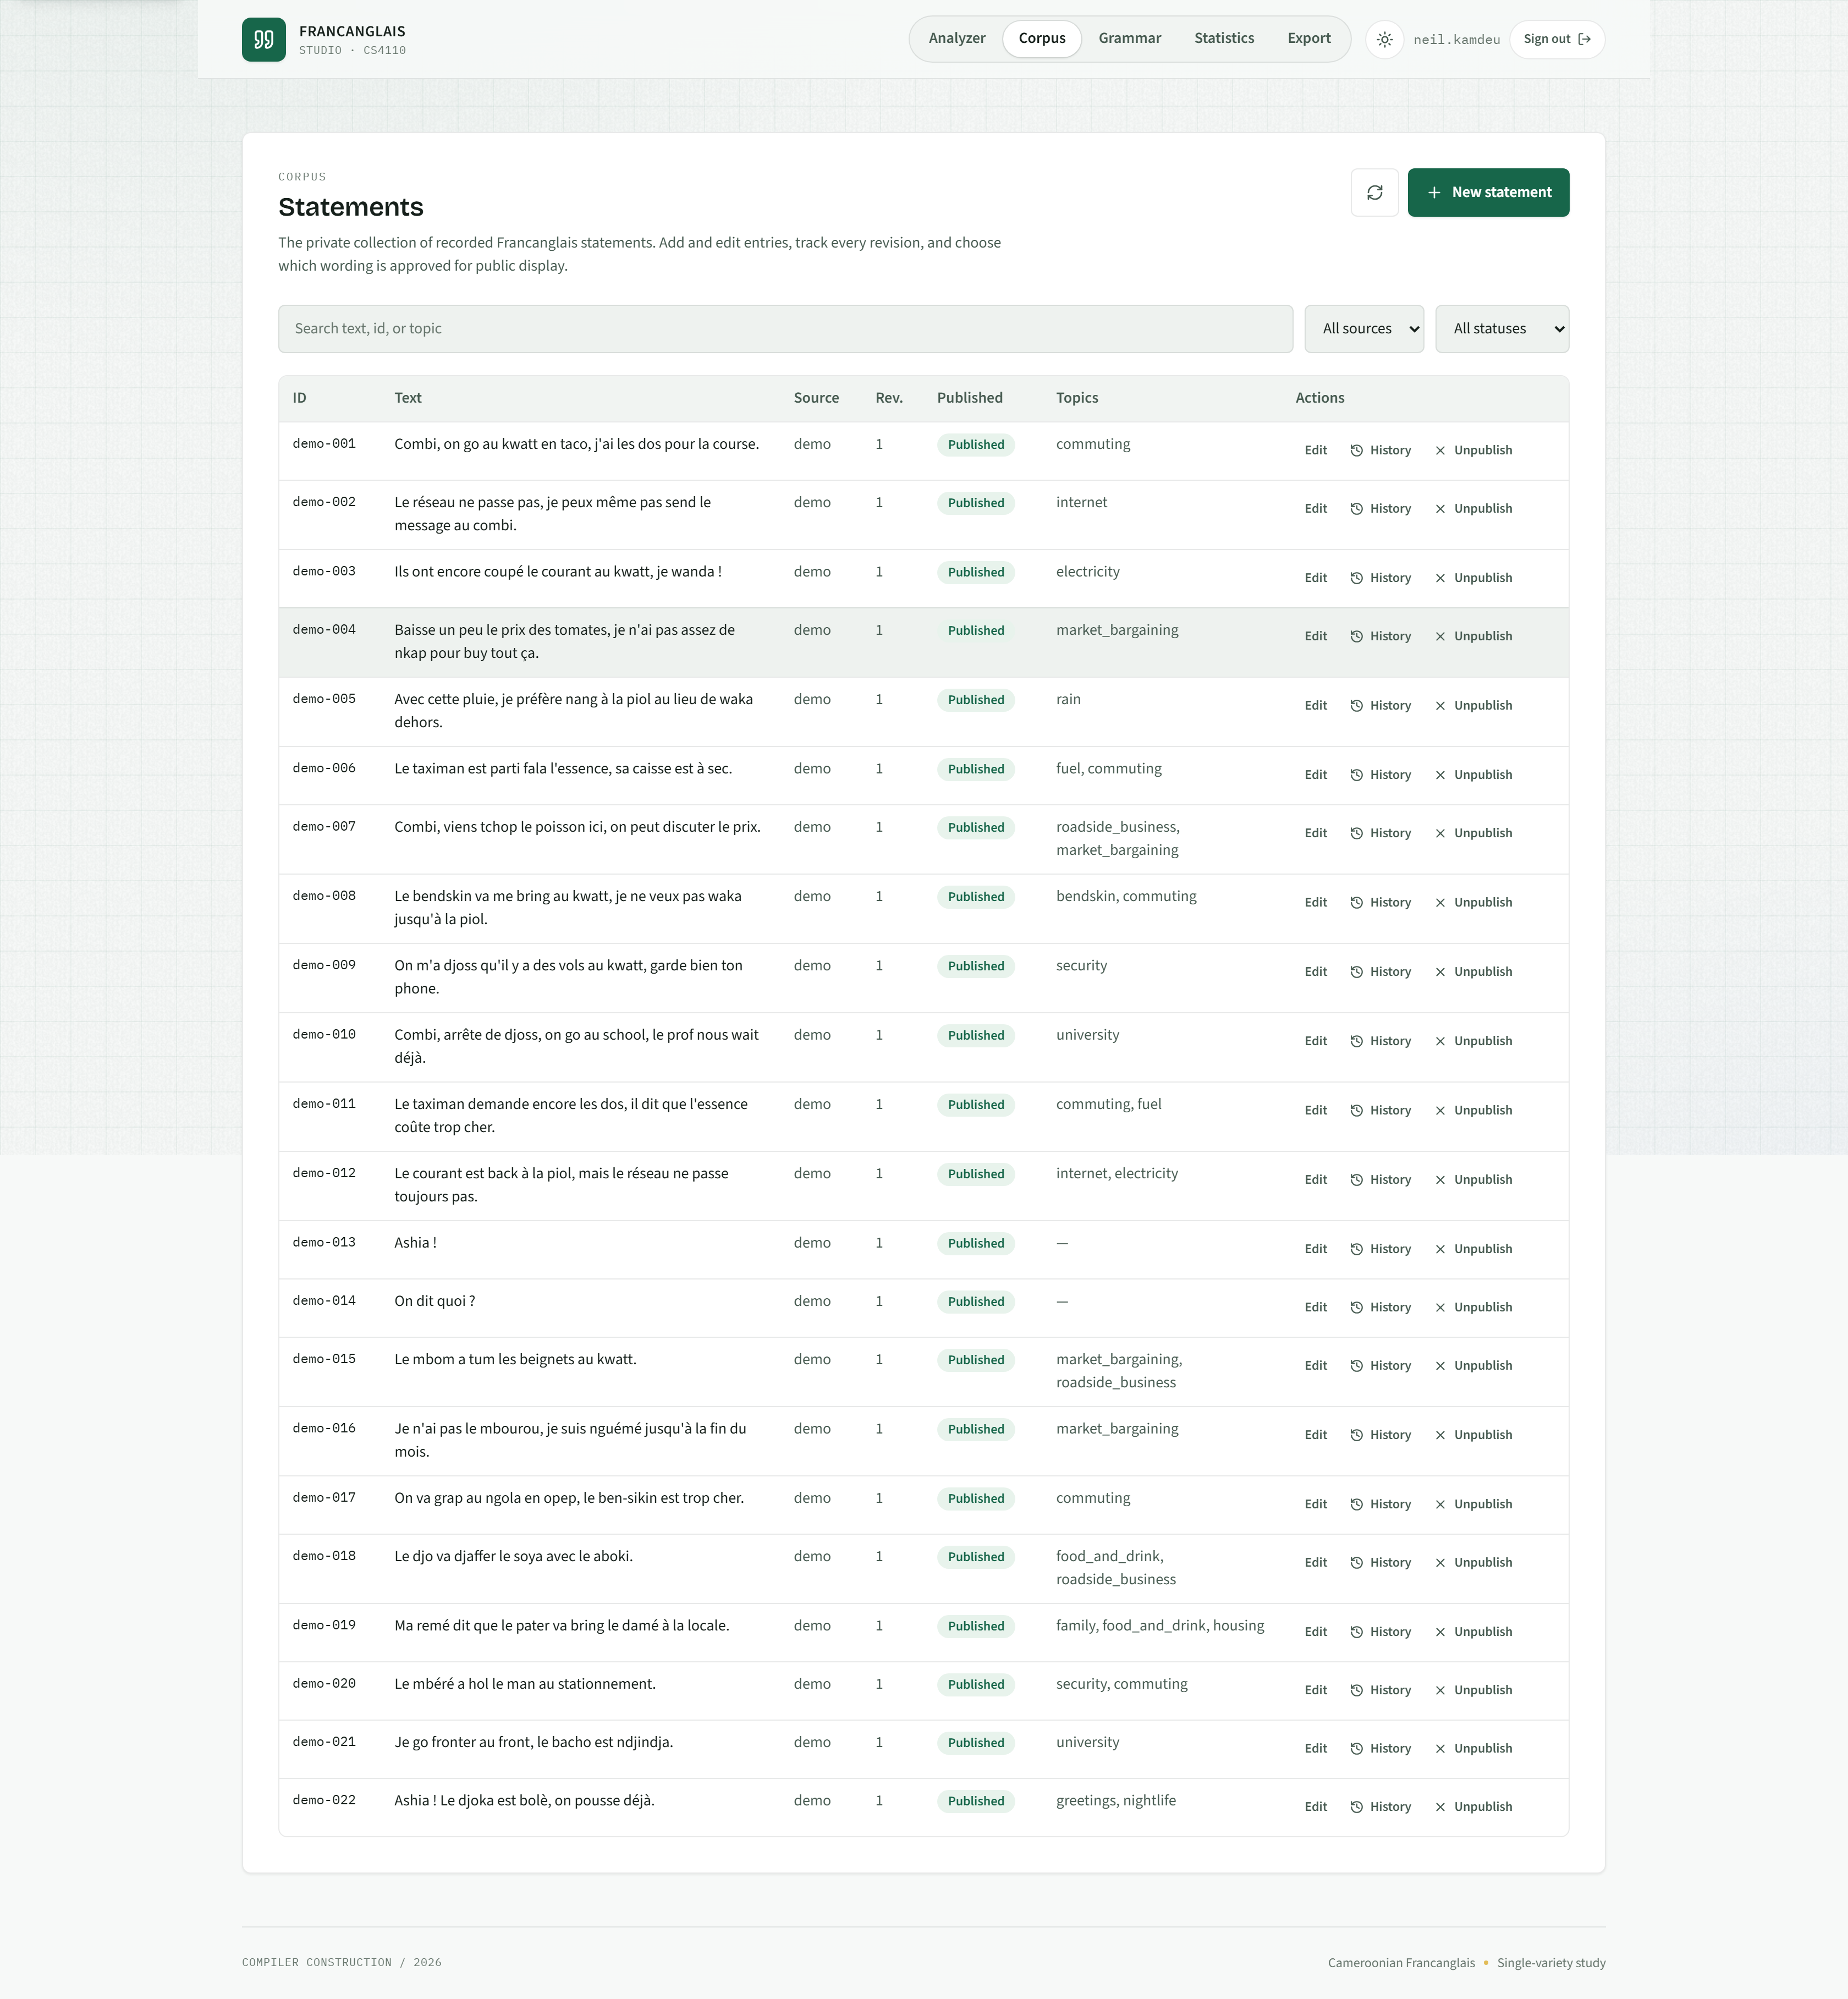
\includegraphics[width=\linewidth]{figures/shot-corpus.png}
  \end{minipage}
  \caption{Left: incremental search filtering the \LexiconTotal\ lexicon entries as the
  user types. Right: the corpus manager, showing per-record source kind, revision number,
  publication state and detected topics.}
\end{figure}
